% !TeX program = xelatex
% C3 midterm defense deck based on ZJU-Beamer-Template.
\PassOptionsToPackage{quiet}{fontspec}
\PassOptionsToPackage{dvipsnames}{xcolor}
\PassOptionsToPackage{fontset=fandol}{ctex}
\documentclass[10pt,aspectratio=169]{beamer}

\usepackage{zju_beamer}
\usepackage{booktabs}
\usepackage{tabularx}
\usepackage{array}
\usepackage{mathtools}

\graphicspath{{./figures/}}
\zjusectioncolor{blue}
\setbeamertemplate{navigation symbols}{}

\definecolor{ZJUBlue}{RGB}{0,63,136}
\definecolor{ZJULight}{RGB}{236,244,252}
\definecolor{ZJUGreen}{RGB}{0,125,117}
\definecolor{WarmGray}{RGB}{90,90,90}

\newcommand{\key}[1]{\textcolor{ZJUBlue}{\textbf{#1}}}
\newcommand{\good}[1]{\textcolor{ZJUGreen}{\textbf{#1}}}
\newcommand{\R}{\mathbb{R}}
\newcommand{\E}{\mathbb{E}}
\newcommand{\argmax}{\operatorname*{arg\,max}}

\title[C3：数据增强 AutoML 定价]{数据增强 AutoML 市场中的最优定价}
\subtitle{论文理论解读：市场机制、定价算法与学习保证}
\author[张博渊、林润铎、彭博宇]{张博渊、林润铎、彭博宇}
\institute[数据要素市场]{数据要素市场课程 · 中期答辩\\参考论文：\textit{Optimal Pricing for Data-Augmented AutoML Marketplaces}}
\date{2026 年 7 月 18 日}

\begin{document}

\begin{frame}
  \titlepage
\end{frame}

\begin{frame}{汇报主线}
  \tableofcontents
  \vspace{0.5em}
  \begin{block}{核心问题}
    如何把\key{数据获取}与\key{模型定价}合并成一个可计算、可学习、可解释的市场机制？
  \end{block}
\end{frame}

\section{研究问题}

\begin{frame}{核心转变：不卖“原始数据”，而卖“可验证的模型增益”}
  \begin{columns}[T,onlytextwidth]
    \begin{column}{0.48\textwidth}
      \begin{block}{现有做法的错配}
        \begin{itemize}
          \item 原始数据价值\key{依赖具体任务}，买方事前难判断是否有用；
          \item AutoML 按计算时间收费，买方可能为\key{无效搜索}承担成本；
          \item 不同买方对同一性能提升有不同支付意愿。
        \end{itemize}
      \end{block}
    \end{column}
    \begin{column}{0.48\textwidth}
      \begin{block}{论文的定价对象}
        \centering
        \vspace{0.25em}
        \large
        \[
          \Delta q = q(C\leftarrow D\Join A)-q(C_0\leftarrow D)
        \]
        \normalsize
        数据增强与模型搜索共同产生的\key{工具性价值}
      \end{block}
      \begin{alertblock}{机制载体}
        平台预先公布价格曲线
        \[
          x: q\in\mathcal Q \longmapsto x(q)\ge 0,
        \]
        对所有买方一视同仁，按最终购买的性能档位收费。
      \end{alertblock}
    \end{column}
  \end{columns}
\end{frame}

\section{市场机制}

\begin{frame}{市场把数据发现、模型搜索与定价接成一个闭环}
  \begin{itemize}
    \item 买方只需提交任务、初始训练数据和评估方式；平台在外部数据池中寻找增广特征与模型。
    \item 发现引擎持续输出性能轨迹，定价引擎将其转换为“\key{性能—价格}”菜单。
  \end{itemize}
  \vspace{0.25em}
  \begin{center}
    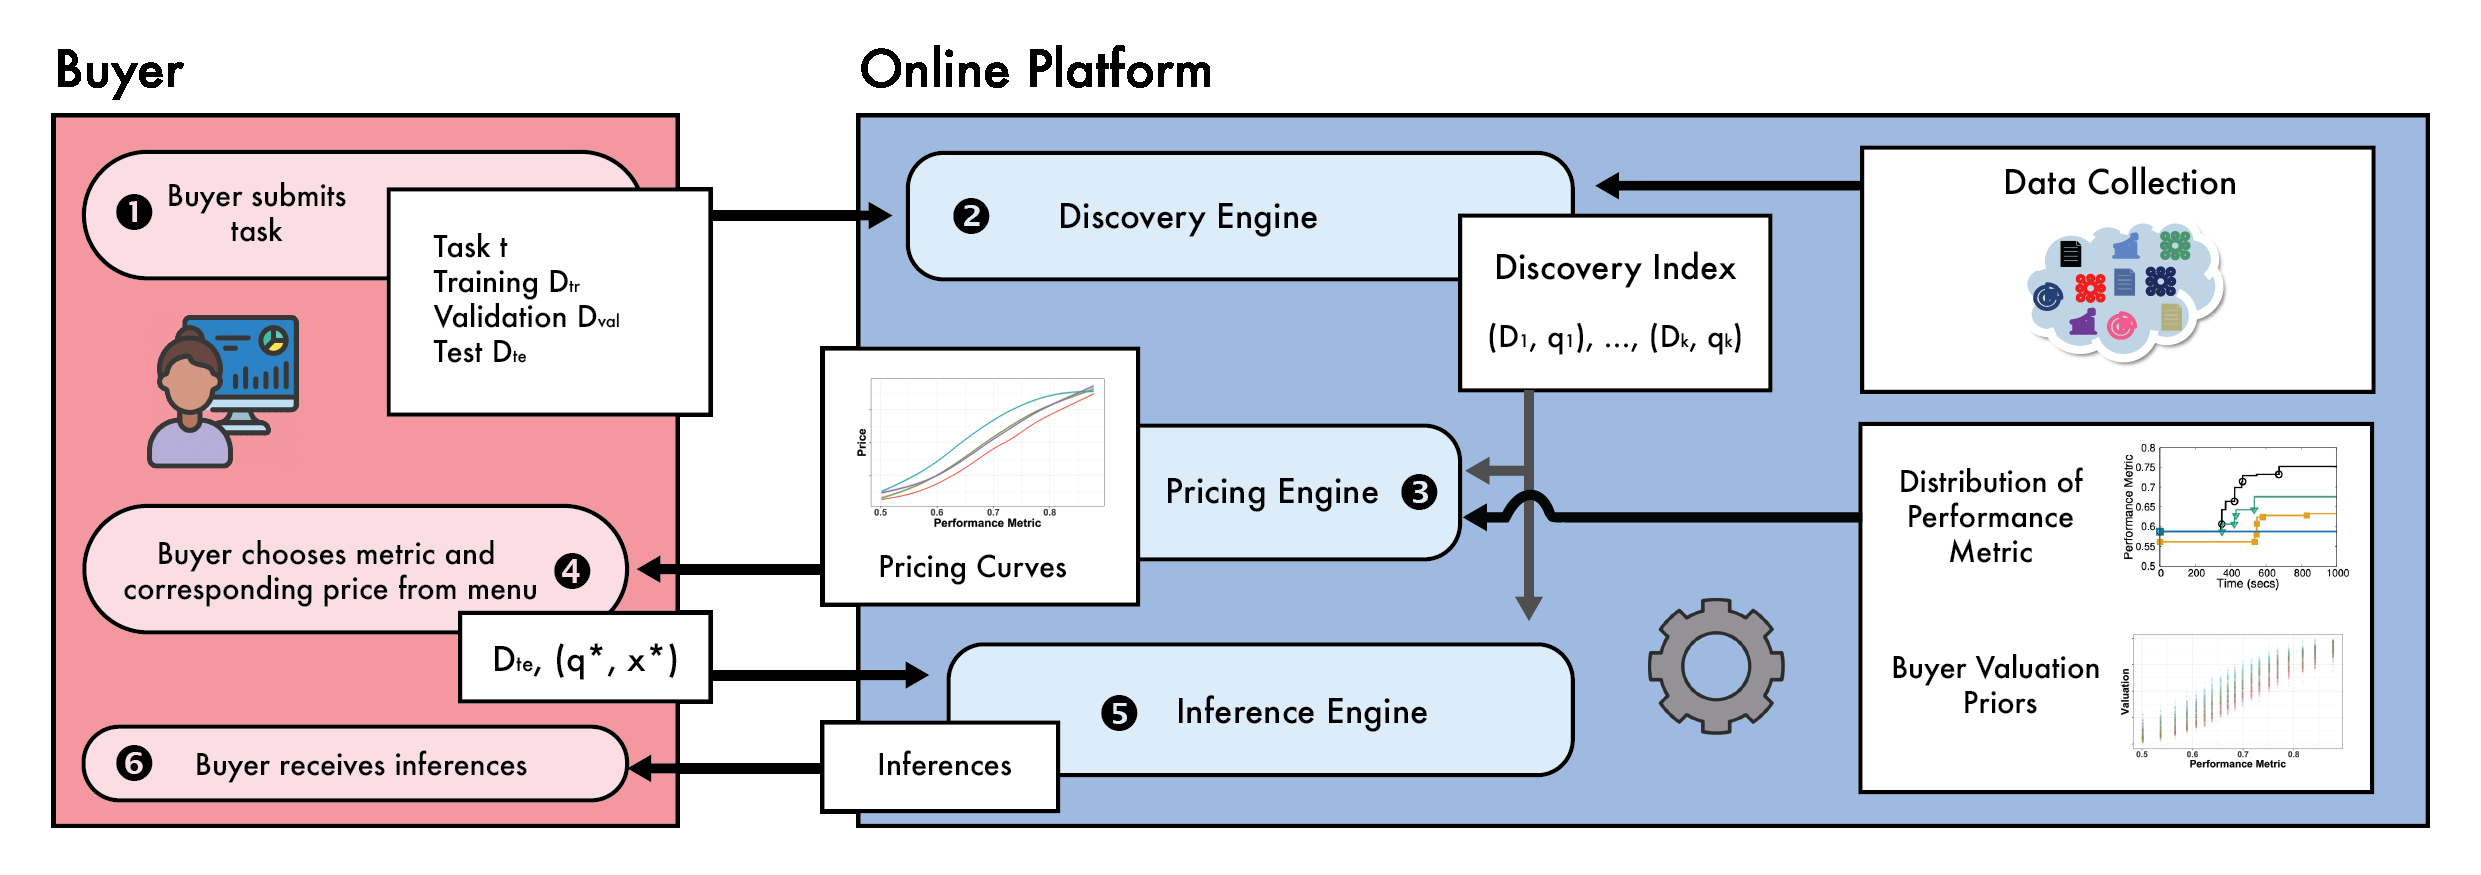
\includegraphics[width=0.88\linewidth]{paper_architecture.png}
  \end{center}
\end{frame}

\begin{frame}{公开价格曲线把三类不确定性收进同一模型}
  \small
  \renewcommand{\arraystretch}{1.18}
  \begin{tabularx}{\linewidth}{>{\bfseries\color{ZJUBlue}}l X}
    \toprule
    符号 & 含义 \\
    \midrule
    $\mathcal Q$ & 离散化的模型性能集合；当前观测为 $q_t\in\mathcal Q$，性能允许暂时下降。\\
    $P^t(q'\mid q)$ & 时变马尔可夫转移矩阵；刻画从当前性能到下一期性能的搜索动态。\\
    $c,T$ & 单位时间真实发现成本与最长搜索期数。\\
    $\theta\sim\mu$ & 买方私有类型及其先验分布；$v^\theta(q)$ 是类型 $\theta$ 对性能 $q$ 的价值。\\
    $x(q)$ & 平台事前公布的统一价格曲线。\\
    \bottomrule
  \end{tabularx}
  \vspace{0.15em}
  \begin{block}{买方效用}
    \centering
    \large
    $u^\theta(q,\tau)=v^\theta(q)-x(q)-c\tau$
  \end{block}
\end{frame}

\begin{frame}{一次交易是一条“观察—继续/停止—购买”路径}
  \begin{columns}[T,onlytextwidth]
    \begin{column}{0.24\textwidth}
      \begin{block}{1. 进入前}
        平台公开 $x(q)$、成本 $c$ 与性能演化指导 $P^t$。
      \end{block}
    \end{column}
    \begin{column}{0.24\textwidth}
      \begin{block}{2. 搜索中}
        每期看到最新 $q_t$；较差结果也会展示，形成多档选择。
      \end{block}
    \end{column}
    \begin{column}{0.24\textwidth}
      \begin{block}{3. 自主决策}
        买方比较立即停止收益与继续搜索的期望收益。
      \end{block}
    \end{column}
    \begin{column}{0.24\textwidth}
      \begin{block}{4. 退出或购买}
        选择已见过的最佳净剩余档位；保留不购买的外部选项。
      \end{block}
    \end{column}
  \end{columns}
  \vspace{0.8em}
  \begin{alertblock}{关键机制性质}
    价格不依赖买方主动报告，减少策略性误报空间；买方仍通过\key{停止时点}表达自己的真实支付意愿。
  \end{alertblock}
\end{frame}

\section{最优定价}

\begin{frame}{买方最优响应是“相关收益版”的 Pandora's Box}
  \begin{columns}[T,onlytextwidth]
    \begin{column}{0.55\textwidth}
      \centering
      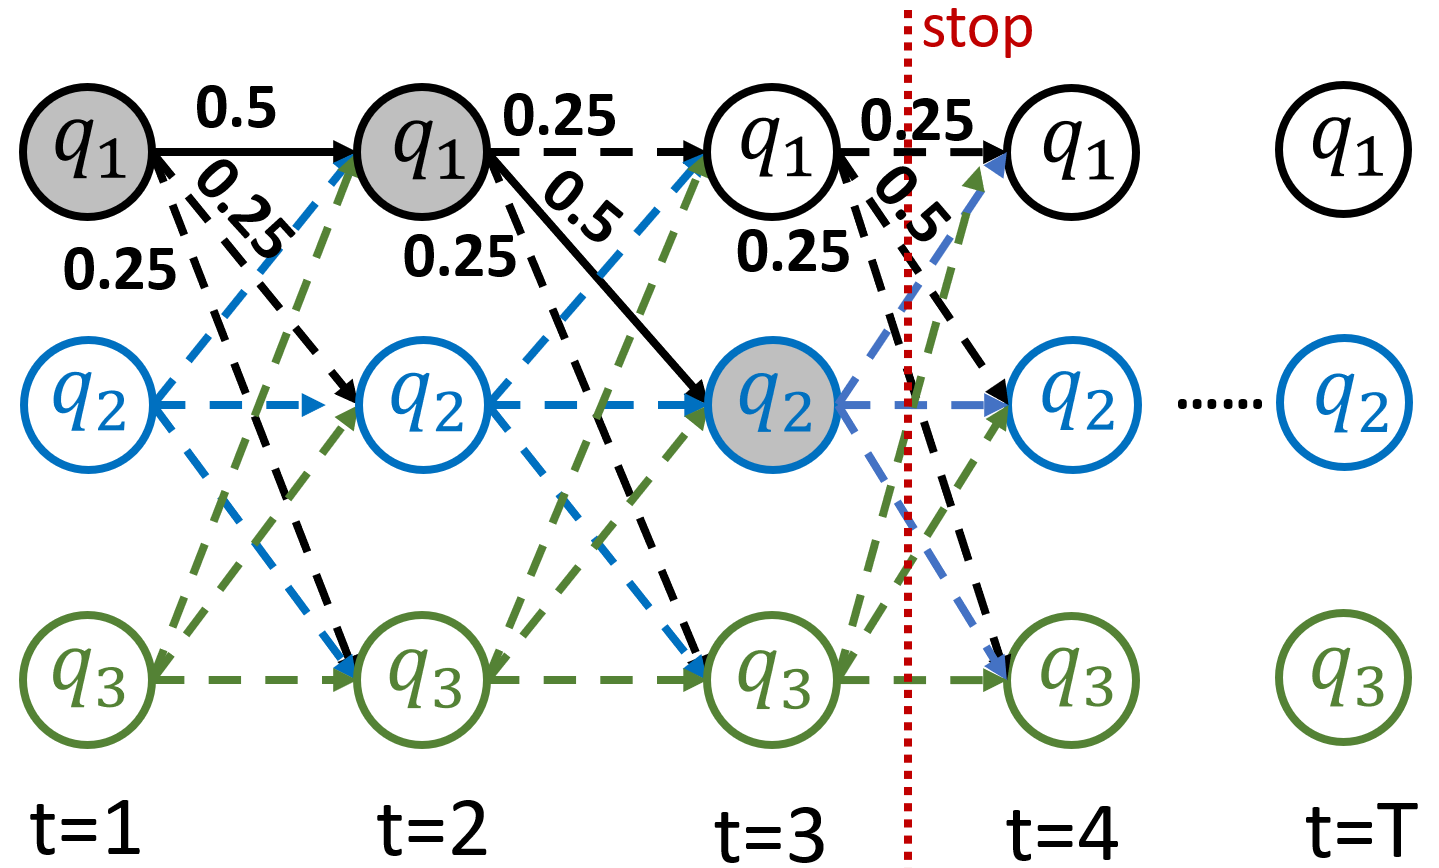
\includegraphics[width=0.96\linewidth]{paper_markov.png}
    \end{column}
    \begin{column}{0.42\textwidth}
      \begin{block}{与经典模型的差异}
        \begin{itemize}
          \item 下一期收益不独立，而依赖当前 $q_t$；
          \item 决策必须记住“历史最佳净剩余”；
          \item 有限时域 $T$ 与逐期真实成本 $c$。
        \end{itemize}
      \end{block}
      \begin{alertblock}{停止规则}
        若\key{立即停止效用}不低于\key{继续搜索的期望效用}，则停止；否则进入下一期。
      \end{alertblock}
    \end{column}
  \end{columns}
\end{frame}

\begin{frame}{一个三维 DP 足以给出最优停止策略}
  \begin{block}{状态定义}
    $(q_1,q_2,t)$：$q_1$ 是历史上净剩余最高的性能档位，$q_2$ 是当前性能，$t$ 是时间。
  \end{block}
  \vspace{0.2em}
  \small
  令
  \[
    S_\theta(q,t)=v^\theta(q)-x(q)-ct,\qquad
    B_\theta(q_1,q)=\argmax_{r\in\{q_1,q\}}\{v^\theta(r)-x(r)\}.
  \]
  则 Bellman 递推为
  \[
    \Phi_\theta(q_1,q_2,t)=
    \max\left\{
      S_\theta(q_1,t),
      \sum_{q\in\mathcal Q}P^{t+1}(q\mid q_2)
      \Phi_\theta\!\left(B_\theta(q_1,q),q,t+1\right)
    \right\}.
  \]
  \begin{alertblock}{命题 4.1}
    状态数为 $|\mathcal Q|^2T$，每个状态可常数时间更新，因此最优策略可在
    \good{$O(|\mathcal Q|^2T)$} 时间内求得。
  \end{alertblock}
\end{frame}

\begin{frame}{平台面对双层优化：价格先行，买方随后最优响应}
  \begin{block}{经验轨迹上的定价问题}
    \centering
    \large
    \[
      \max_{x\ge 0}\;\sum_{\theta}\mu(\theta)\frac{1}{m}
      \sum_{s\in\mathcal S}x\!\left(q^*(\theta,x,s)\right),
      \qquad
      q^*=\argmax_{q\in s}\bigl[v^\theta(q)-x(q)\bigr].
    \]
  \end{block}
  \begin{itemize}
    \item 外层选择价格曲线 $x$ 最大化期望收入；内层买方按净效用选择性能档位。
    \item $x(q)\times\mathbb 1\{q=q^*\}$ 同时含连续变量与离散选择，不能直接交给线性求解器。
    \item 论文在定理 4.2 中采用“发现成本相对价值可忽略”的假设，将问题转成样本轨迹上的菜单选择。
  \end{itemize}
\end{frame}

\begin{frame}{MILP 用四类变量把买方选择与平台收入线性化}
  \small
  \renewcommand{\arraystretch}{1.08}
  \begin{tabularx}{\linewidth}{>{\bfseries\color{ZJUBlue}}p{0.13\linewidth} p{0.18\linewidth} X}
    \toprule
    变量 & 类型 & 经济含义 \\
    \midrule
    $x(q)$ & 连续 & 平台对性能档位 $q$ 的公开价格。\\
    $z_{\theta s q}$ & 0--1 & 类型 $\theta$ 在轨迹 $s$ 上是否选择 $q$。\\
    $a_{\theta s}$ & 连续 & 该买方在该轨迹上的最大净效用。\\
    $y_{\theta s q}$ & 连续 & 线性化 $x(q)z_{\theta s q}$，即实际收入贡献。\\
    \bottomrule
  \end{tabularx}
  \vspace{0.1em}
  \begin{columns}[T,onlytextwidth]
    \begin{column}{0.49\textwidth}
      \begin{block}{选择约束}
        \[
          \sum_{q\in s}z_{\theta s q}=1,
        \]
        \[
          0\le a_{\theta s}-[v^\theta(q)-x(q)]
          \le M(1-z_{\theta s q}).
        \]
      \end{block}
    \end{column}
    \begin{column}{0.49\textwidth}
      \begin{block}{收入线性化}
        \[
          y\le x,\quad y\le Mz,
        \]
        \[
          y\ge x-M(1-z),\quad y\ge 0.
        \]
      \end{block}
    \end{column}
  \end{columns}
\end{frame}

\begin{frame}{有限样本轨迹仍能学到近优价格曲线}
  \small
  \begin{alertblock}{定理 4.2：PAC 型保证}
    若买方价值上界为 $b$，且发现成本相对价值可忽略，当样本数满足
    \[
      m\;\ge\;\frac{b^2}{2\varepsilon^2}\ln\frac{2}{\delta},
    \]
    MILP 输出的 $\widehat x$ 以至少 $1-2\delta$ 的概率满足
    \[
      g(\widehat x,\mathcal S)\ge g(x^*,\mathcal S)-\varepsilon.
    \]
  \end{alertblock}
  \begin{columns}[T,onlytextwidth]
    \begin{column}{0.49\textwidth}
      \begin{block}{证明路线}
        \begin{enumerate}
          \item MILP 在样本上精确求最优菜单；
          \item 单个任务收入落在 $[0,b]$；
          \item Hoeffding 不等式控制经验收入与总体收入之差。
        \end{enumerate}
      \end{block}
    \end{column}
    \begin{column}{0.49\textwidth}
      \begin{block}{直观含义}
        精度提高一倍，样本量约增至四倍；机制无需准确写出完整转移矩阵，只需采样真实性能轨迹。
      \end{block}
    \end{column}
  \end{columns}
\end{frame}

\section{学习与结论}

\begin{frame}{未知买方先验可由“停止行为”反向学习}
  \small
  \begin{block}{Bayesian 更新}
    观察第 $t$ 轮买方在 $y^{(t)}$ 停止后，类型后验为
    \[
      w^{(t)}(\theta_i)=
      \frac{\Pr(y^{(t)}\mid \theta_i,x^{(t)})\,\mu^{(t)}(\theta_i)}
      {\sum_j\Pr(y^{(t)}\mid \theta_j,x^{(t)})\,\mu^{(t)}(\theta_j)},
      \qquad
      \mu^{(t+1)}=(1-\eta_t)\mu^{(t)}+\eta_t w^{(t)}.
    \]
  \end{block}
  \begin{columns}[T,onlytextwidth]
    \begin{column}{0.49\textwidth}
      \begin{block}{可识别性}
        若不同类型在某些价格下产生不同停止分布，重复交互即可逐步区分类型。
      \end{block}
    \end{column}
    \begin{column}{0.49\textwidth}
      \begin{alertblock}{定理 5.2：鲁棒性}
        若 $\|\mu-\mu^*\|_2\le\varepsilon$ 且 $\|P-P^*\|_2\le\varepsilon$，则
        \[
          \mathrm{CEE}(\mu,P)=O(\varepsilon),
        \]
        即估计误差只造成线性级收入损失。
      \end{alertblock}
    \end{column}
  \end{columns}
\end{frame}

\begin{frame}{发现引擎为定价机制生成可随时停止的性能轨迹}
  \begin{columns}[T,onlytextwidth]
    \begin{column}{0.47\textwidth}
      \begin{block}{直接搜索不可行}
        若增广集合为 $\mathcal P$、模型集合为 $\mathcal M$，穷举需要训练
        \[
          O\!\left(2^{|\mathcal P|}|\mathcal M|\right)
        \]
        个模型。即便用 Metam 排序增广，逐轮测试全部模型仍需
        $O(|\mathcal M|\log|\mathcal P|)$ 次训练。
      \end{block}
    \end{column}
    \begin{column}{0.50\textwidth}
      \begin{alertblock}{论文的联合发现算法}
        \begin{enumerate}
          \item 用 Metam 聚类并选择候选增广；
          \item 将每个模型视作一个 Exp3 臂；
          \item 每轮只采样并训练\key{一个模型}；
          \item 用当前性能作为奖励更新模型权重。
        \end{enumerate}
      \end{alertblock}
    \end{column}
  \end{columns}
  \vspace{0.5em}
  \begin{block}{与定价机制的接口}
    算法具备 anytime 性质：每轮输出一个 $q_t$，买方可随时停止；序列 $(q_1,\ldots,q_T)$ 正是 DP 与 MILP 所需的性能轨迹。
  \end{block}
\end{frame}

\begin{frame}{论文的理论结论依赖四个关键建模边界}
  \begin{enumerate}
    \item \key{性能动态：}$\mathcal Q$ 有限离散，且未来性能只依赖当前 $q_t$ 与时间 $t$；转移矩阵 $P^t$ 可公开或估计。
    \item \key{买方偏好：}类型空间有限、价值有界；不同类型需要通过停止行为具有可识别性。
    \item \key{价格形式：}平台面对所有买方公布同一条按性能收费的价格曲线，不依赖买方主动报告。
    \item \key{计算假设：}定理 4.2 在发现成本相对价值可忽略时给出 MILP 的 PAC 保证；一般成本下的误差影响由定理 5.2 控制。
  \end{enumerate}
  \vspace{0.45em}
  \begin{alertblock}{论文聚焦的范围}
    核心是“买方停止决策 + 平台收入最优定价”；上游数据供应者之间如何分配收入并不是本文的主要机制设计问题。
  \end{alertblock}
\end{frame}

\begin{frame}{论文的答案：围绕模型结果设计一条可计算的价格曲线}
  \begin{enumerate}
    \item \key{卖什么：}不直接给原始数据定价，而给数据增强后的模型性能定价；
    \item \key{买方如何选择：}将搜索视为相关收益的 Pandora's Box，用 DP 求最优停止；
    \item \key{平台如何定价：}用 MILP 显式编码买方最优响应，并从有限轨迹学习近优价格；
    \item \key{未知信息如何处理：}由停止行为学习买方先验，估计误差只带来线性级收入损失；
    \item \key{性能轨迹从哪里来：}Metam 搜索增广，Exp3 在每轮选择一个模型，支持 anytime 交互。
  \end{enumerate}
  \vspace{0.6em}
  \begin{alertblock}{核心贡献}
    数据发现、模型搜索、买方停止与平台定价被统一为一个与 AutoML 接口兼容的市场机制。
  \end{alertblock}
  \vfill
  \centering\large Q\&A
\end{frame}

\appendix
\section*{附录}

\begin{frame}{附录 A：MILP 完整形式}
  \scriptsize
  \[
    \max_{x,a,y,z}\quad
    \sum_{\theta}\mu(\theta)\frac{1}{m}
    \sum_{s\in\mathcal S}\sum_{q\in s}y(\theta,s,q)
  \]
  \[
  \begin{aligned}
    \text{s.t.}\quad
    &0\le a_{\theta,s}-\bigl[v^\theta(q)-x(q)\bigr]
      \le M\bigl(1-z(\theta,s,q)\bigr), &&\forall\theta,s,q,\\
    &\sum_{q\in s}z(\theta,s,q)=1, &&\forall\theta,s,\\
    &y(\theta,s,q)\le x(q),\qquad
      y(\theta,s,q)\le Mz(\theta,s,q), &&\forall\theta,s,q,\\
    &y(\theta,s,q)\ge x(q)-M\bigl(1-z(\theta,s,q)\bigr), &&\forall\theta,s,q,\\
    &x\ge0,\qquad y\ge0,\qquad z\in\{0,1\}.&
  \end{aligned}
  \]
  \begin{block}{Big-$M$ 的作用}
    当 $z=1$ 时强制 $a=v^\theta(q)-x(q)$ 且 $y=x(q)$；当 $z=0$ 时只保留上界，并令 $y=0$。
  \end{block}
\end{frame}

\begin{frame}{附录 B：联合增广—模型发现算法}
  \small
  \begin{enumerate}
    \item 初始化增广解集 $\mathcal T\leftarrow\varnothing$，并令每个模型权重 $w(M)=1$；
    \item 从候选数据集中选择增广 $T_i\subseteq\mathcal P$；
    \item 以
      \[
        \Pr(M)=(1-\gamma)\frac{w(M)}{\sum_{M'\in\mathcal M}w(M')}
        +\frac{\gamma}{|\mathcal M|}
      \]
      采样模型 $M_i$；
    \item 在 $D_{\mathrm{in}}\Join T_i$ 上训练 $M_i$，以性能指标作为重要性加权奖励并更新 $w(M_i)$；
    \item 达到停止条件后，返回观测效用最高的增广，并在该增广上选择最佳模型。
  \end{enumerate}
  \begin{alertblock}{设计目的}
    每轮只训练一个模型，同时保留探索概率 $\gamma$；因此能够边搜索边汇报性能，为买方的最优停止决策提供在线轨迹。
  \end{alertblock}
\end{frame}

\begin{frame}[allowframebreaks]{参考文献}
  \nocite{*}
  \bibliographystyle{unsrt}
  \bibliography{references}
\end{frame}

\end{document}
